%% abtex2-modelo-artigo.tex, v-1.9.7 laurocesar
%% Copyright 2012-2018 by abnTeX2 group at http://www.abntex.net.br/
%%
%% This work may be distributed and/or modified under the
%% conditions of the LaTeX Project Public License, either version 1.3
%% of this license or (at your option) any later version.
%% The latest version of this license is in
%%   http://www.latex-project.org/lppl.txt
%% and version 1.3 or later is part of all distributions of LaTeX
%% version 2005/12/01 or later.
%%
%% This work has the LPPL maintenance status `maintained'.
%%
%% The Current Maintainer of this work is the abnTeX2 team, led
%% by Lauro César Araujo. Further information are available on
%% http://www.abntex.net.br/
%%
%% This work consists of the files abntex2-modelo-artigo.tex and
%% abntex2-modelo-references.bib
%%

% ------------------------------------------------------------------------
% ------------------------------------------------------------------------
% abnTeX2: Modelo de Artigo Acadêmico em conformidade com
% ABNT NBR 6022:2018: Informação e documentação - Artigo em publicação
% periódica científica - Apresentação
% ------------------------------------------------------------------------
% ------------------------------------------------------------------------

\documentclass[
	% -- opções da classe memoir --
	article,			% indica que é um artigo acadêmico
	11pt,				% tamanho da fonte
	oneside,			% para impressão apenas no recto. Oposto a twoside
	a4paper,			% tamanho do papel.
	% -- opções da classe abntex2 --
	%chapter=TITLE,		% títulos de capítulos convertidos em letras maiúsculas
	%section=TITLE,		% títulos de seções convertidos em letras maiúsculas
	%subsection=TITLE,	% títulos de subseções convertidos em letras maiúsculas
	%subsubsection=TITLE % títulos de subsubseções convertidos em letras maiúsculas
	% -- opções do pacote babel --
	english,			% idioma adicional para hifenização
	brazil,				% o último idioma é o principal do documento
	sumario=tradicional
	]{abntex2}


% ---
% PACOTES
% ---

% ---
% Pacotes fundamentais
% ---
\usepackage{lmodern}			% Usa a fonte Latin Modern
\usepackage[T1]{fontenc}		% Selecao de codigos de fonte.
\usepackage[utf8]{inputenc}		% Codificacao do documento (conversão automática dos acentos)
\usepackage{indentfirst}		% Indenta o primeiro parágrafo de cada seção.
\usepackage{nomencl} 			% Lista de simbolos
\usepackage{color}				% Controle das cores
\usepackage{graphicx}			% Inclusão de gráficos
\usepackage{microtype} 			% para melhorias de justificação
% ---

% ---
% Pacotes adicionais, usados apenas no âmbito do Modelo Canônico do abnteX2
% ---
\usepackage{lipsum}				% para geração de dummy text
% ---


% ---
% Pacotes de citações
% ---
\usepackage[brazilian,hyperpageref]{backref}	 % Paginas com as citações na bibl
\usepackage[alf]{abntex2cite}	% Citações padrão ABNT
% ---

% ----
% Para o comentário de porções largas de código
% ----
\usepackage{comment}

% Para citações de multiplas figuras
\usepackage[brazilian]{cleveref}
\newcommand{\crefrangeconjunction}{ \`{a}\nobreakspace}

% ---
% Configurações do pacote backref
% Usado sem a opção hyperpageref de backref
\renewcommand{\backrefpagesname}{Citado na(s) página(s):~}
% Texto padrão antes do número das páginas
\renewcommand{\backref}{}
% Define os textos da citação
\renewcommand*{\backrefalt}[4]{
	\ifcase #1 %
		Nenhuma citação no texto.%
	\or
		Citado na página #2.%
	\else
		Citado #1 vezes nas páginas #2.%
	\fi}%
% ---

% --- Informações de dados para CAPA e FOLHA DE ROSTO ---
\titulo{Trabalho da Disciplina CMC 103 -- Machine Learning}
\tituloestrangeiro{}

\autor{
Crisitano Gurgel de Castro\thanks{Inmetro, (21) 2679 9799, cgcastro at inmetro gov br}
}

\local{Duque de Caxias}
\data{\today}
% ---

% ---
% Configurações de aparência do PDF final

% alterando o aspecto da cor azul
\definecolor{blue}{RGB}{41,5,195}

% informações do PDF
\makeatletter
\hypersetup{
     	%pagebackref=true,
		%pdftitle={\@title},
		%pdfauthor={\@author},
    	%pdfsubject={Modelo de artigo científico com abnTeX2},
	   % pdfcreator={LaTeX with abnTeX2},
		%pdfkeywords={abnt}{latex}{abntex}{abntex2}{atigo científico},
		colorlinks=true,       		% false: boxed links; true: colored links
    	linkcolor=blue,          	% color of internal links
    	citecolor=blue,        		% color of links to bibliography
    	filecolor=magenta,      		% color of file links
		urlcolor=blue,
		bookmarksdepth=4
}
\makeatother
% ---

% ---
% compila o indice
% ---
\makeindex
% ---

% ---
% Altera as margens padrões
% ---
\setlrmarginsandblock{3cm}{3cm}{*}
\setulmarginsandblock{3cm}{3cm}{*}
\checkandfixthelayout
% ---

% ---
% Espaçamentos entre linhas e parágrafos
% ---

% O tamanho do parágrafo é dado por:
\setlength{\parindent}{1.3cm}

% Controle do espaçamento entre um parágrafo e outro:
\setlength{\parskip}{0.2cm}  % tente também \onelineskip

% Espaçamento simples
\SingleSpacing

% Definição do comando de questão
% TODO definir comando para ficar não permitir a quebra de página ao meio
\newenvironment{comandoquestao}{\begin{citacao}\textbf{Comando:}}{\end{citacao}}

% Definição matemáticas
\usepackage{siunitx}
\sisetup{output-decimal-marker={,}}

%\renewcommand{\sin}{\operatorname{sen}}
%\let\sin\relax
%\DeclareMathOperator{\sen}{sen}

% ----
% Início do documento
% ----
\begin{document}

% Seleciona o idioma do documento (conforme pacotes do babel)
%\selectlanguage{english}
\selectlanguage{brazil}

% Retira espaço extra obsoleto entre as frases.
\frenchspacing

% ----------------------------------------------------------
% ELEMENTOS PRÉ-TEXTUAIS
% ----------------------------------------------------------

%---
%
% Se desejar escrever o artigo em duas colunas, descomente a linha abaixo
% e a linha com o texto ``FIM DE ARTIGO EM DUAS COLUNAS''.
% \twocolumn[    		% INICIO DE ARTIGO EM DUAS COLUNAS
%
%---

% página de titulo principal (obrigatório)
\maketitle


% titulo em outro idioma (opcional)



% resumo em português
\begin{comment}
\begin{resumoumacoluna}
   Conforme a ABNT NBR 6022:2018, o resumo no idioma do documento é elemento obrigatório.
   Constituído de uma sequência de frases concisas e objetivas e não de uma
   simples enumeração de tópicos, não ultrapassando 250 palavras, seguido, logo
   abaixo, das palavras representativas do conteúdo do trabalho, isto é,
   palavras-chave e/ou descritores, conforme a NBR 6028. (\ldots) As
   palavras-chave devem figurar logo abaixo do resumo, antecedidas da expressão
   Palavras-chave:, separadas entre si por ponto e finalizadas também por ponto.
   \vspace{\onelineskip}
   \noindent
   \textbf{Palavras-chave}: latex. abntex. editoração de texto.
  \end{resumoumacoluna}
\end{comment}



% resumo em inglês

% ]  				% FIM DE ARTIGO EM DUAS COLUNAS
% ---

\begin{center}\smaller
\textbf{Data de submissão}: 13 de novembro de 2024.

\begin{comment}
\textbf{Identificação e disponibilidade}: elemento opcional. Pode ser indicado
o endereço eletrônico, DOI, suportes e outras informações relativas ao acesso.
\end{comment}

\end{center}

% ----------------------------------------------------------
% ELEMENTOS TEXTUAIS
% ----------------------------------------------------------
\textual

% ----------------------------------------------------------
% Introdução
% ----------------------------------------------------------
\section{Introdução}

Na presente atividade, se propõe-se a conduzir uma análise de uma série de tarefas, cada uma focalizando diferentes parâmetros e hiperparâmetros associados às redes neurais artificiais. Com o objetivo principal de delinear a influência desses elementos técnicos sobre as propriedades comportamentais das redes neurais e obter elucidação de possíveis critérios e processos envolvidos na seleção desses parâmetros em aplicações práticas.

% ----------------------------------------------------------
% Seção de explicações
% ----------------------------------------------------------
\section{Tarefas Propostas}

Para as presentes tarefas, uma rede neural foi dada como exemplo. Tal rede é 
treinada para um conjunto de dados ${(x_i, y_i)}$ que refletem o comportamento 
de uma senóide $y_i = \sin(x_i) + r_i$. Um ruído $r_i$ foi adicionado a 
cada 
medição de forma a refletir uma coleta de dados no mundo real com uma incerteza 
de medição associada

\subsection{Tarefa 1}

\begin{comandoquestao}
   Nesta tarefa, você explorará o impacto de diferentes funções de ativação no desempenho da rede neural. A função de ativação controla como os neurônios transformam os dados de entrada, e diferentes funções podem influenciar a capacidade de aprendizado da rede.
\end{comandoquestao}

A rede neural dada como exemplo utiliza a função Gelu como função de ativação nas camadas intermediárias. Vericamos o comportamento do erro de treinamento em relação ao número de épocas de treinamento (figura \ref{tarefa01:gelu:treinamento}), bem como a comparação dos dados previstos pela rede dados em relação aos dados de treinamento na figura \ref{tarefa01:gelu:predicoes}.

\begin{figure}[htb]
	\label{teste}
	\centering
	\begin{minipage}{0.45\textwidth}
	\centering
	\caption{Gelu: Treinamento} \label{tarefa01:gelu:treinamento}
	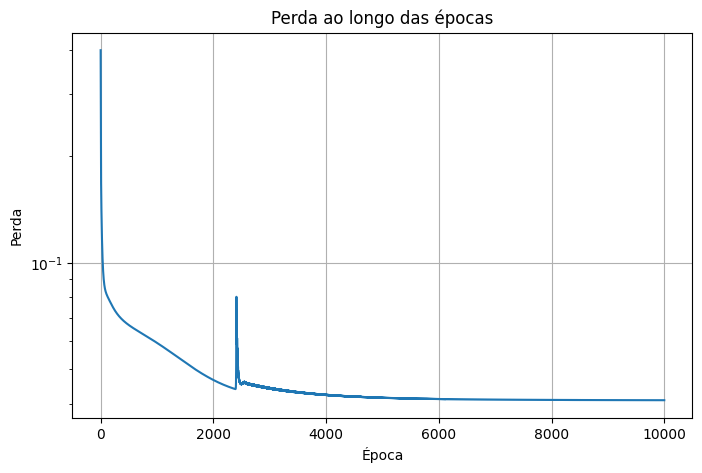
\includegraphics[width=\textwidth]{./0803_imgs/png-241111-212601400-7995113924505873963.png}
	%\legend{Fonte: Gerado peloComando da atividade}
	\end{minipage}
	\hfill
	\begin{minipage}{0.45\textwidth}
	\centering
	\caption{Gelu: predições} \label{tarefa01:gelu:predicoes}
	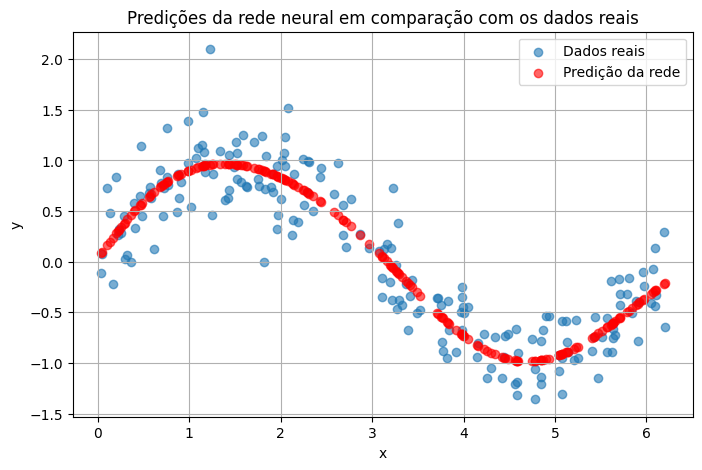
\includegraphics[width=\textwidth]{./0803_imgs/png-241111-212606975-12044568718402292765.png}
	%\legend{Fonte: \citeonline[p. 24]{araujo2012}}
	\end{minipage}
\end{figure}

Para a presente tarefa modificamos a função de ativação das camadas intermediárias para sigmóide, obtendo os resultados mostrados nas figuras


\begin{figure}[htb]
	\label{teste}
	\centering
	\begin{minipage}{0.45\textwidth}
	\centering
	\caption{Gelu: Treinamento} \label{tarefa01:gelu:treinamento}
	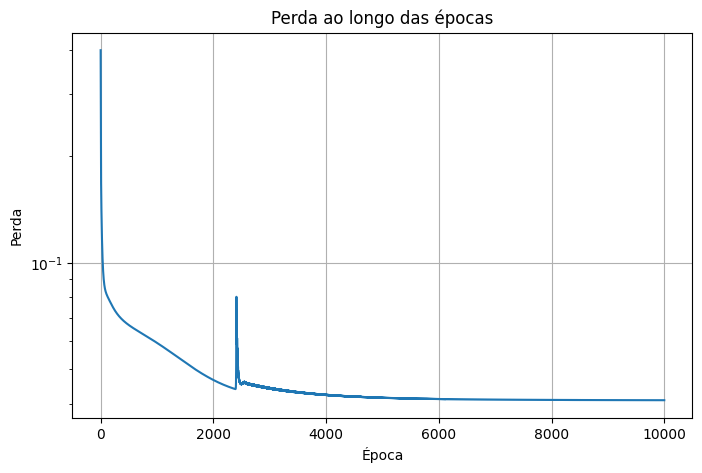
\includegraphics[width=\textwidth]{./0803_imgs/png-241111-212601400-7995113924505873963.png}
	%\legend{Fonte: Gerado peloComando da atividade}
	\end{minipage}
	\hfill
	\begin{minipage}{0.45\textwidth}
	\centering
	\caption{Gelu: predições} \label{tarefa01:gelu:predicoes}
	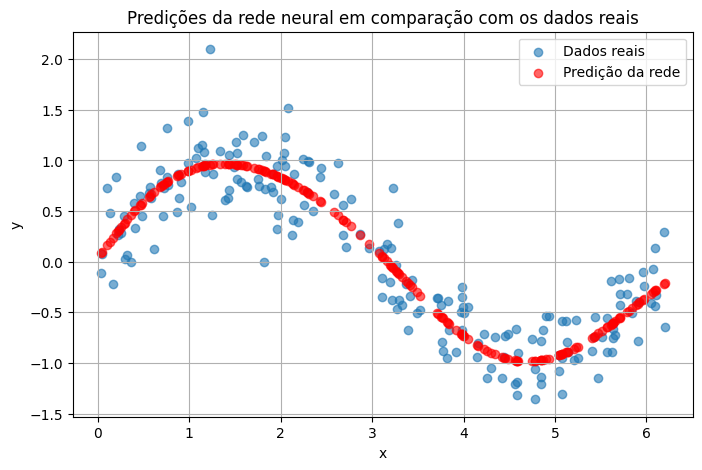
\includegraphics[width=\textwidth]{./0803_imgs/png-241111-212606975-12044568718402292765.png}
	%\legend{Fonte: \citeonline[p. 24]{araujo2012}}
	\end{minipage}
\end{figure}

\subsection{Tarefa 02 -- Variação do Número de Épocas}

\begin{comandoquestao}
    Objetivo. Analisar como a quantidade de épocas de treinamento influencia o desempenho da rede neural na aproximação da função seno. Observaremos como diferentes números de épocas afetam a convergência da perda e a qualidade das predições da rede.
\end{comandoquestao}

No presente treinamento, treinamos 4 redes neurais distintas. Todas tem a mesma 
características, mesmo modelo, mesmas funções de ativação nas camadas 
intermediárias (gelu) e mesma taxa de aprendizado. No entanto cada uma delas 
foi treinada com um número diferente de épocas. Vemos os resultados nas 
\cref{tarefa02:1000:predicoes,tarefa02:5000:predicoes,tarefa02:10000:predicoes,tarefa02:20000:predicoes}
 a seguir. Na \cref{tarefa02:figura:curvas} tem-se as curvas de erros durante o 
treinamento para as redes neurais. Na \cref{tarefa02:tabela:perdas} vemos as 
perdas para um mesmo conjunto de dados de teste referentes às diferentes redes 
neurais.


\begin{figure}[htb]
	\centering
	\begin{minipage}{0.45\textwidth}
	\centering
	\caption{Treinando com 1k épocas.}\label{tarefa02:1000:predicoes}
	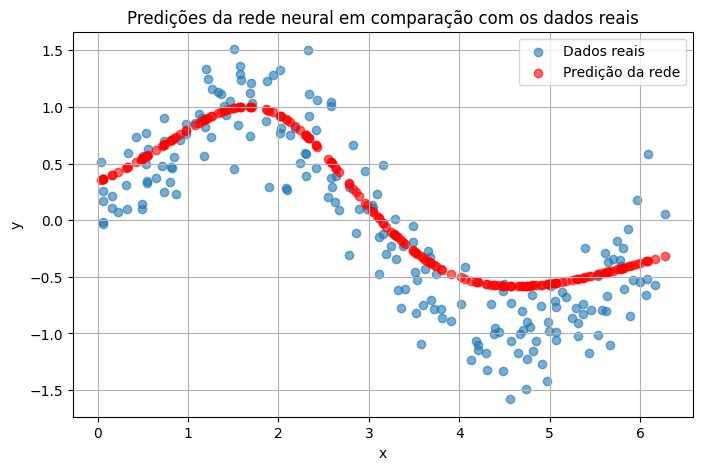
\includegraphics[width=\textwidth]{./0803_imgs/png-241110-154527304-12037654268696582542.png}
	%\legend{Fonte: Gerado peloComando da atividade}
	\end{minipage}
	\hfill
	\begin{minipage}{0.45\textwidth}
	\centering
	\caption{Treinando com 5k épocas.}\label{tarefa02:5000:predicoes}
	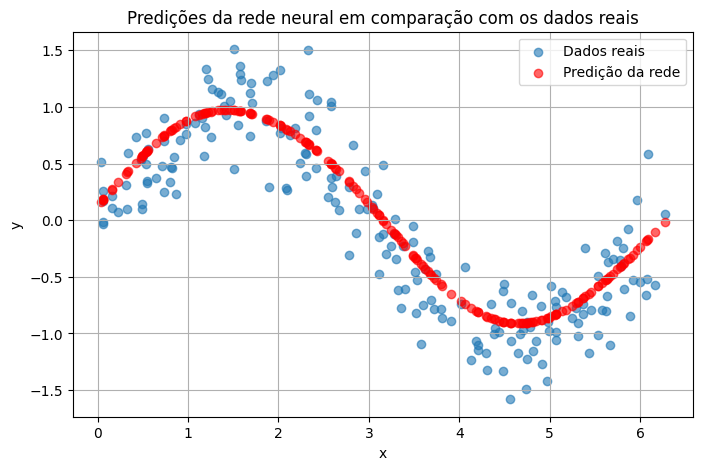
\includegraphics[width=\textwidth]{./0803_imgs/png-241110-154628196-17784737572676737911.png}
	%\legend{Fonte: \citeonline[p. 24]{araujo2012}}
	\end{minipage}
    \vspace{1Ex}
    \begin{minipage}{0.45\textwidth}
        \centering
        \caption{Treinando com 10k épocas.}\label{tarefa02:10000:predicoes}
        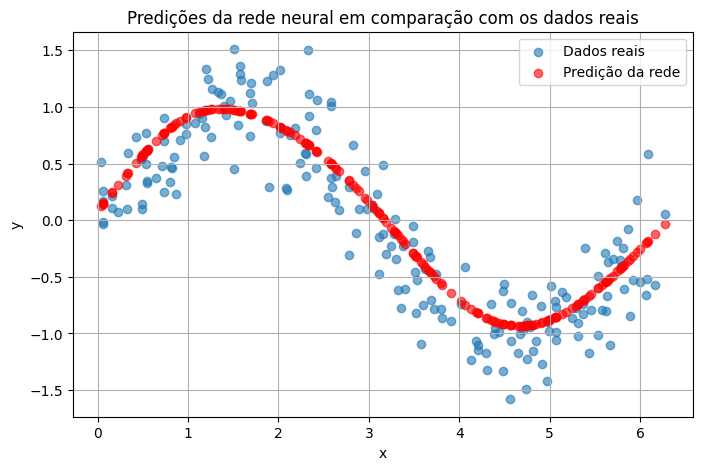
\includegraphics[width=\textwidth]{./0803_imgs/png-241110-154812342-18762265025268743.png}
        %\legend{Fonte: \citeonline[p. 24]{araujo2012}}
    \end{minipage}
	\hfill
	\begin{minipage}{0.45\textwidth}
	\centering
	\caption{Treinando com 20k épocas.}\label{tarefa02:20000:predicoes}
	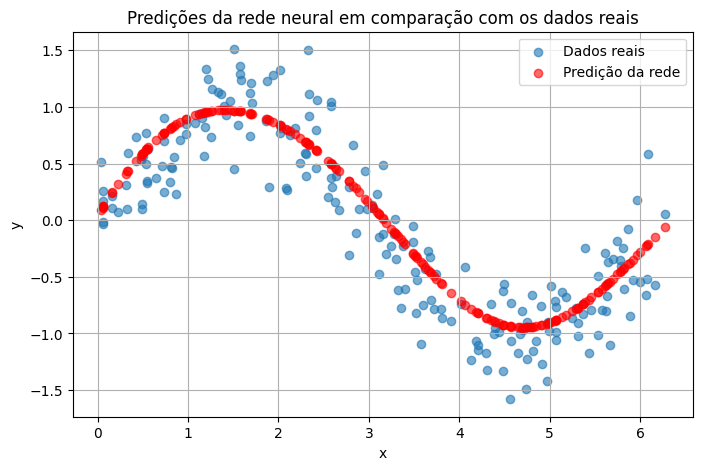
\includegraphics[width=\textwidth]{./0803_imgs/png-241110-155300412-9439382542521307108.png}
	%\legend{Fonte: \citeonline[p. 24]{araujo2012}}
	\end{minipage}
\end{figure}

\begin{figure}
	\centering
	\caption{Curvas de perdas durante o treinamento para as diferentes 
	redes}\label{tarefa02:figura:curvas}
	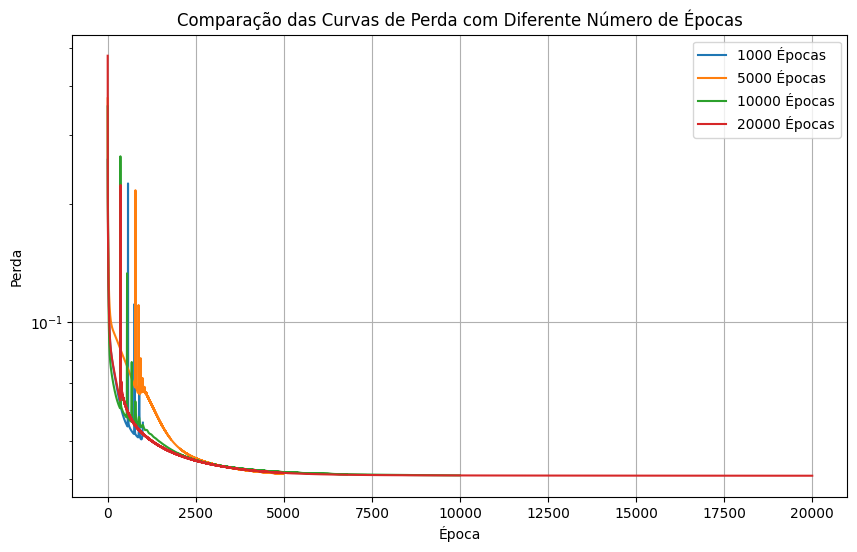
\includegraphics[width=0.7\linewidth]{./0803_imgs/png-241110-160937603-16503693892993531452.png}
\end{figure}

\begin{table}[htb]
	\caption{Perda de teste para as diferentes redes neurais}
	\centering
	\label{tarefa02:tabela:perdas}
\begin{tabular}{c | c}
	Rede Neural & Perda com dados de teste \\
	1k épocas  &  0.06468 \\
	5k épocas  &  0.04504 \\
	10k épocas &  0.04528 \\
	20k épocas &  0.04492
\end{tabular}
\end{table}

Após 5000 épocas de treinamento, foi observado que as redes neurais apresentam 
erros muito próximos uns dos outros. Isso indica que, a partir desse ponto, 
aumentar ainda mais o número de épocas de treinamento não traz melhorias 
significativas na capacidade preditiva das redes. Este achado é importante, 
pois sugere que as redes alcançaram um nível de desempenho máximo e que o 
treinamento adicional pode não ser benéfico.

Um caso especial que chama a atenção é a rede neural treinada com apenas 1000 
épocas. Esta rede exibe um erro de previsão significativamente maior do que as 
outras redes, indicando um caso de "underfitting". Underfitting ocorre quando 
um modelo é muito simples para capturar os padrões complexos nos dados, 
resultando em um desempenho de previsão inferior.

Uma observação secundária interessante é a comparação entre a rede treinada com 
a função de ativação Gelu por 1000 épocas e a rede treinada com a função de 
ativação sigmóide. Parece que ambas as redes têm capacidades preditivas 
semelhantes, apesar da diferença na função de ativação e no número de épocas de 
treinamento. Isso pode sugerir que, neste caso específico, a função de ativação 
Gelu com menos épocas de treinamento pode alcançar um desempenho comparável ao 
sigmóide.

Em resumo, esta análise destaca a importância de monitorar o desempenho das 
redes neurais em diferentes pontos do treinamento. Mostra que o underfitting 
pode ocorrer com menos épocas de treinamento e que diferentes funções de 
ativação podem ter impactos variados no desempenho do modelo. Os resultados 
também sugerem que, após um certo número de épocas, a melhoria no desempenho da 
rede neural pode ser marginal, indicando que a otimização adicional pode não 
ser necessária.

\subsection{Tarefa 03}

\begin{comandoquestao}
Objetivo. Investigar como diferentes taxas de aprendizado 
(\texttt{learning\_rate}) afetam a 
convergência e o desempenho da rede neural. Analisaremos como a velocidade e a 
estabilidade do treinamento variam com a alteração dessa taxa.
\end{comandoquestao}

Nessa atividade treinamos uma mesma rede neural com os mesmos dados de testes, 
variando apenas a taxa de aprendizado ($\alpha$) e verificando o seu 
comportamento durante 
o treinamento e a capacidade de previsão da rede. Treinamos as redes para 
$\alpha = 0,001 | 0,01 | 0,05 | 0,1$. A evolução do erro durante o treinamento 
para as redes é mostrada na \cref{tarefa03:tabela:curvas}. As 
capacidades de previsão das redes são mostradas nas figuras 

\begin{figure}[tbh]
	\centering
	\caption{Curvas de perda durante treinamento (modificando $\alpha$)}
	\label{tarefa03:tabela:curvas}
	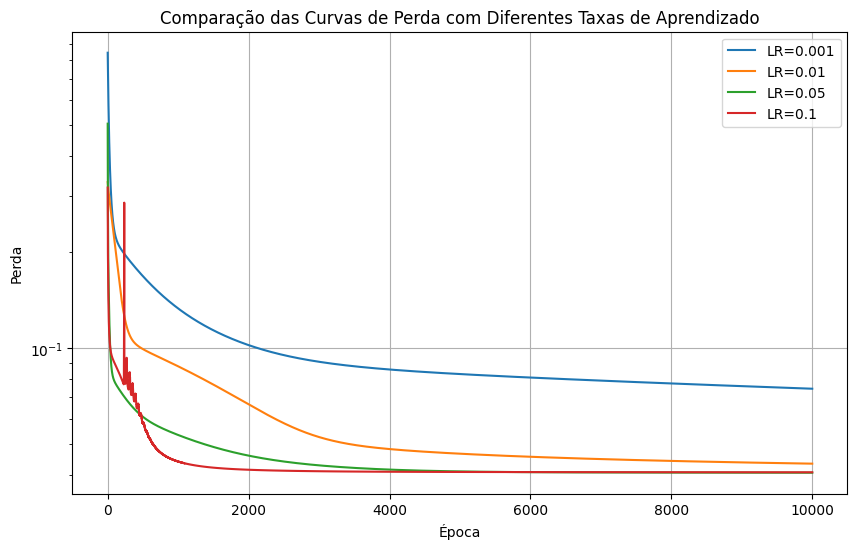
\includegraphics[width=0.7\linewidth]{./0803_imgs/png-241110-180530307-18269409044321663699.png}
\end{figure}


\begin{figure}[htb]
	\centering
	\begin{minipage}{0.45\textwidth}
		\centering
		\caption{$\alpha = 0,001$}\label{tarefa03:0001:predicoes}
		
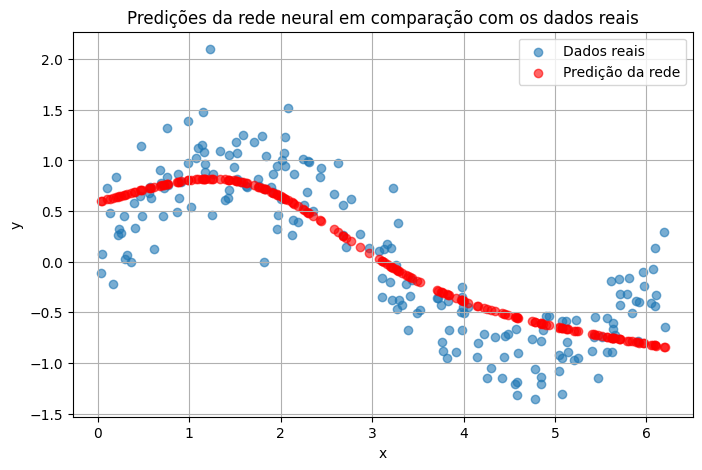
\includegraphics[width=\textwidth]{./0803_imgs/png-241110-175032242-2586281422306343440.png}
		%\legend{Fonte: Gerado peloComando da atividade}
	\end{minipage}
	\hfill
	\begin{minipage}{0.45\textwidth}
		\centering
		\caption{$\alpha = 0,01$}\label{tarefa03:001:predicoes}
		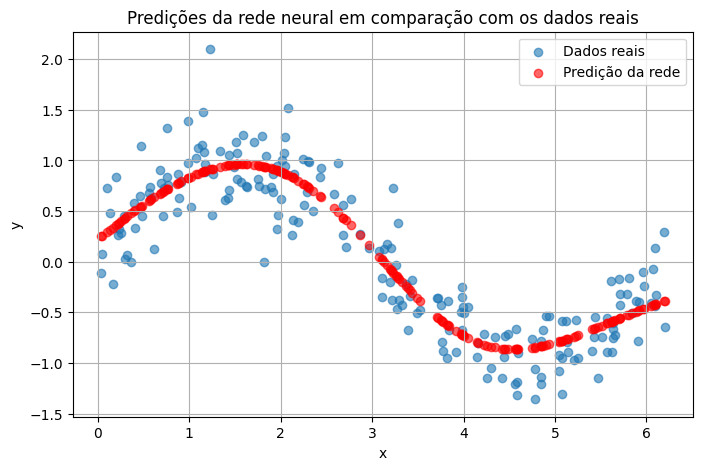
\includegraphics[width=\textwidth]{./0803_imgs/png-241110-175254024-1064294634935646228.png}
		%\legend{Fonte: \citeonline[p. 24]{araujo2012}}
	\end{minipage}
%	\vspace{1Ex}
%	\begin{minipage}{0.45\textwidth}
%		\centering
%		\caption{{$\alpha = 0,05$}\label{tarefa03:005:predicoes}
%		%\includegraphics[width=\textwidth]{./0803_imgs/}
%		%\legend{Fonte: \citeonline[p. 24]{araujo2012}}
%	\end{minipage}
%	\hfill
%	\begin{minipage}{0.45\textwidth}
%		\centering
%		\caption{{$\alpha = 0,1$}\label{tarefa03:01:predicoes}
%		%\includegraphics[width=\textwidth]{./0803_imgs/}
%		%\legend{Fonte: \citeonline[p. 24]{araujo2012}}
%	\end{minipage}
\end{figure}
\subsection{Tarefa 04 -- Ajuste do Número de Neurônios por Camada}

\begin{comandoquestao}
	Objetivo: Avaliar como a quantidade de neurônios em cada camada oculta 
	influencia a capacidade de aprendizagem e a performance da rede neural. 
	Exploraremos diferentes arquiteturas para entender o impacto da 
	complexidade da 	rede.
\end{comandoquestao}

Foram realizados experimentos de treinamento com quatro diferentes 
configurações de neurônios nas camadas ocultas, mantendo o número de épocas 
constante em 10000. A primeira configuração com $[1, 5, 5, 5, 1]$ neurônios em 
cada camada resultou em uma perda de treinamento de $\approx 0,04058$. A 
segunda configuração com $[1, 10, 10, 10, 1]$ neurônios produziu uma perda de 
$\approx 0.04076$. A terceira configuração com $[1, 20, 20, 20, 1]$ neurônios 
resultou em 
uma perda de $\approx 0.04071$, e a quarta configuração com $[1, 50, 50, 50, 
1]$ neurônios 
teve uma perda de $\approx 0.04078$. As curvas de treinamento podem ser vistas 
na \cref{fig:tarefa04:curvas}

\begin{figure}[tbh]
	\centering
	\caption{Curvas de aprendizados para diferentes configurações da rede}
	\label{fig:tarefa04:curvas}
	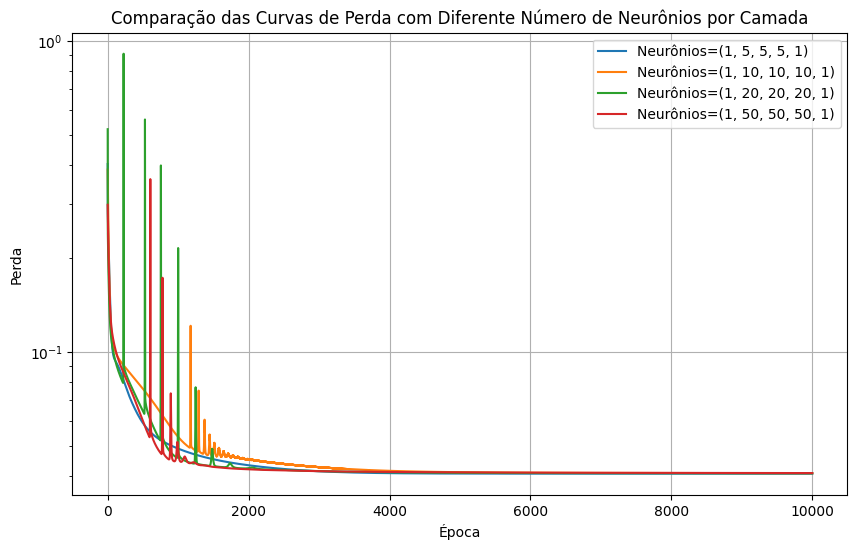
\includegraphics[width=0.7\linewidth]{./0803_imgs/png-241110-190844867-15619254497487317135.png}
\end{figure}

O efeito no tempo de treinamento para cada arquitetura pode ser visto na 
\cref{fig:tarefa04:tempo}. É importante notar que, conforme 
veremos mais adiante e com base na quantidade de dados disponível, não é 
necessário ter camadas muito densas com muitos neurônios.

\begin{figure}[tbh]
	\centering
	\caption{Tempo de treinamento de acordo com a arquitetura da rede}
	\label{fig:tarefa04:tempo}
	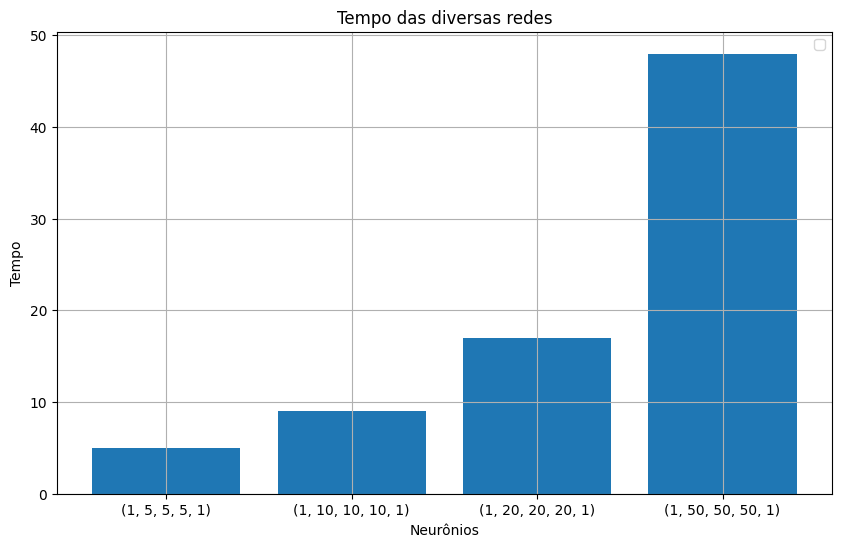
\includegraphics[width=0.7\linewidth]{./0803_imgs/png-241110-190809211-3985790047096570638.png}
\end{figure}

As predições das redes são mostradas nas 
\cref{fig:tarefa04:5:predicoes,fig:tarefa04:10:predicoes,fig:tarefa04:20:predicoes,fig:tarefa04:50:predicoes}
A configuração mais simples, com menos neurônios, apresenta uma boa 
convergência e uma curva de perda suave, sem muitas oscilações. Isso 
implica que, para este conjunto de dados específico, uma arquitetura de rede 
neural menos complexa pode ser suficiente para obter bons resultados.



\begin{figure}[htb]
	\centering
	\begin{minipage}{0.45\textwidth}
		\centering
		\caption{Configuração $[1, 5, 5, 5, 1]$}\label{fig:tarefa04:5:predicoes}
		
		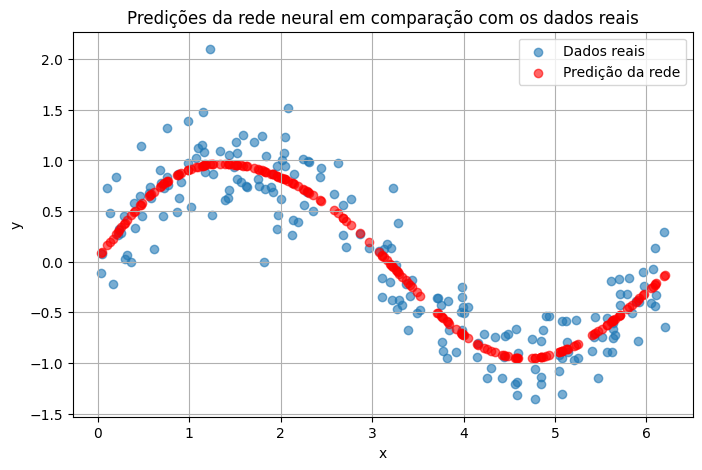
\includegraphics[width=\textwidth]{./0803_imgs/0052_tarefa04/png-241110-190441034-11876360900706154495.png}
		%\legend{Fonte: Gerado peloComando da atividade}
	\end{minipage}
	\hfill
	\begin{minipage}{0.45\textwidth}
		\centering
		\caption{Configuração $[1, 10, 10, 10, 
		1]$}\label{fig:tarefa04:10:predicoes}
		
		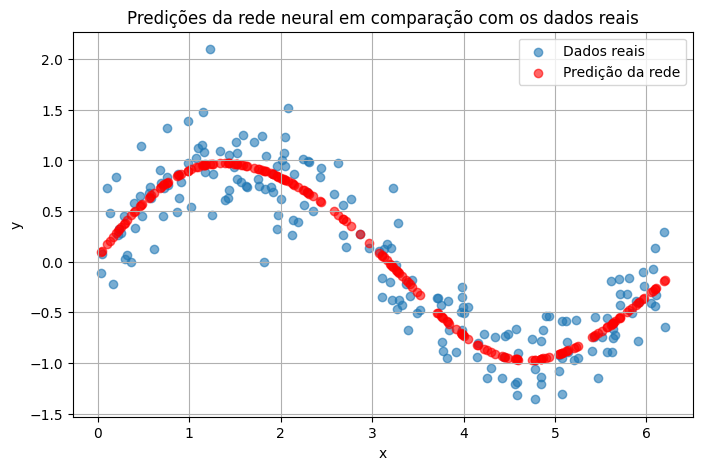
\includegraphics[width=\textwidth]{./0803_imgs/0052_tarefa04/png-241110-190600007-13238267918468901506.png}
		%\legend{Fonte: \citeonline[p. 24]{araujo2012}}
	\end{minipage}
	\vspace{2Ex}
	\begin{minipage}{0.45\textwidth}
		\centering
		\caption{Configuração $[1, 20, 20, 20, 
		1]$}\label{fig:tarefa04:20:predicoes}
		
		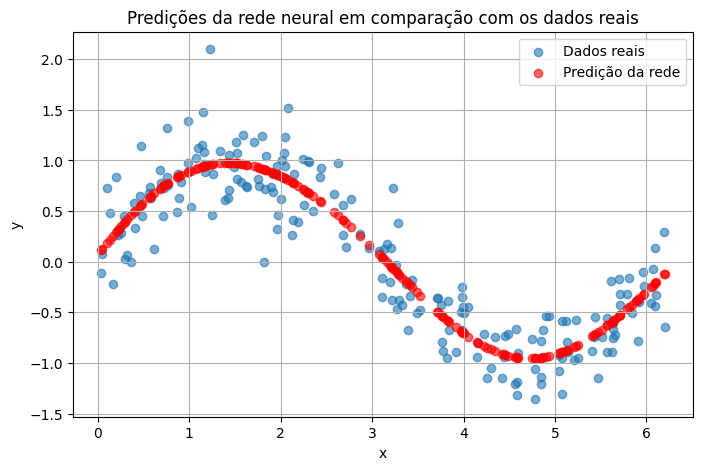
\includegraphics[width=\textwidth]{./0803_imgs/0052_tarefa04/png-241110-190633260-11858406457361919316.png}
		%		%\legend{Fonte: \citeonline[p. 24]{araujo2012}}
	\end{minipage}
	\hfill
	\begin{minipage}{0.45\textwidth}
		\centering
		\caption{Configuração $[1, 50, 50, 50, 
		1]$}\label{fig:tarefa04:50:predicoes}
		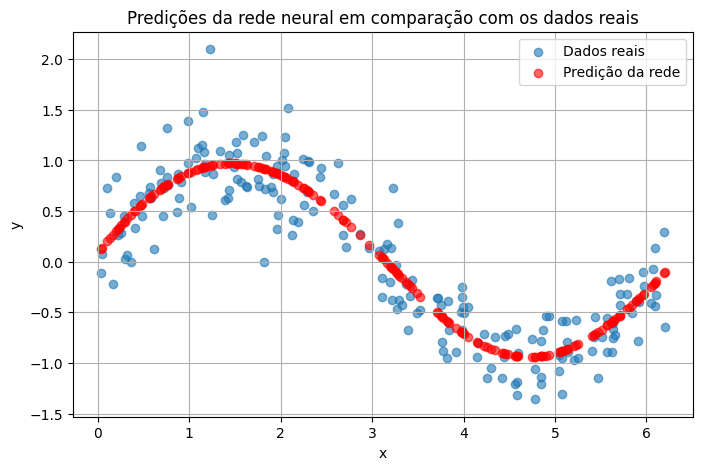
\includegraphics[width=\textwidth]{./0803_imgs/0052_tarefa04/png-241110-190650933-14380430249431153222.png}
		%\legend{Fonte: \citeonline[p. 24]{araujo2012}}
	\end{minipage}
\end{figure}


Em resumo, esta análise destaca a importância de considerar a complexidade da 
arquitetura da rede neural em relação à quantidade de dados disponíveis. Em 
alguns casos, uma rede neural mais simples pode convergir bem e fornecer 
resultados comparáveis a redes mais profundas e complexas. A escolha da 
arquitetura ideal depende dos dados específicos e dos objetivos do problema em 
questão.


\subsection{Tarefa 5: Introdução de Ruído nos Dados de Treinamento}

\begin{comandoquestao}
Objetivo: Investigar como diferentes níveis de ruído nos dados de treinamento 
afetam a performance e a generalização da rede neural. Avaliaremos a robustez 
do modelo frente a dados ruidosos.
\end{comandoquestao}

Foram realizados experimentos de treinamento com quatro níveis diferentes de 
ruído adicionados aos dados: $\sigma=0.0$, $\sigma=0.1$, $\sigma=0.3$ e 
$\sigma=0.5$. O gráfico de treinamento para as diferentes redes é apresentada 
na \cref{fig:tarefas05:curvas}


\begin{figure}[tbh]
	\centering
	\caption{Curvas de aprendizado para diferentes níveis de ruído dos dados de 
	entrada}
	\label{fig:tarefas05:curvas}
	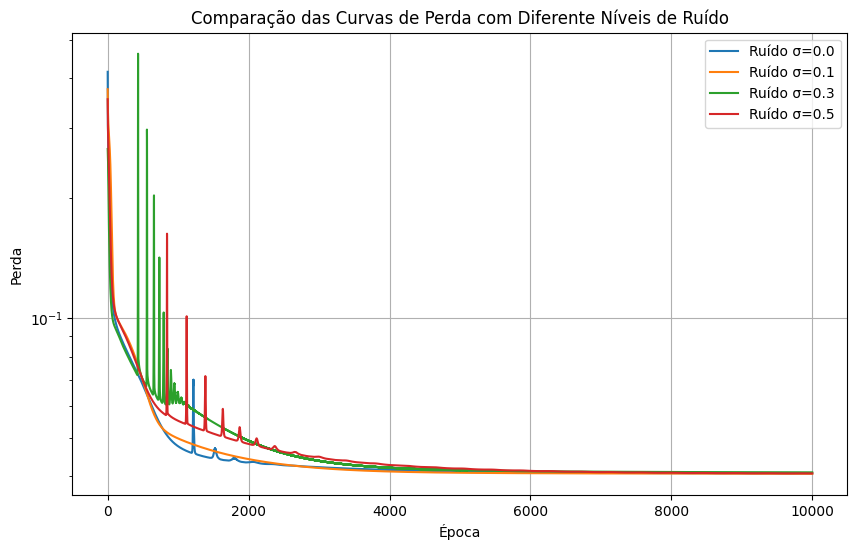
\includegraphics[width=0.7\linewidth]{./0803_imgs/0365_tarefa05/png-241110-193148800-7110775020035268662.png}
\end{figure}


Para $\sigma=0.0$, que 
representa dados sem ruído, os gráficos de perda (loss)
mostram uma convergência suave e rápida, indicando que o modelo está aprendendo 
bem.

Para as redes com níveis de ruídos maiores, a convergência é ligeiramente mais 
lenta e a perda é um pouco maior em comparação com os dados sem ruído. Isso é 
esperado, pois o ruído adiciona complexidade aos dados, tornando a tarefa de 
aprendizagem mais desafiadora.

Com $\sigma=0,3$, a convergência torna-se mais instável, especialmente nas 
primeiras 
épocas do treinamento. A perda oscila mais e leva mais tempo para estabilizar. 
Isso sugere que o modelo está encontrando dificuldades para aprender os padrões 
subjacentes nos 
dados devido ao alto nível de ruído.

Para $\sigma=0,5$, é notável que a convergência parece 
mais estável do que $\sigma=0,3$ nas primeiras épocas, sugerindo que o modelo 
está encontrando maneiras de lidar com o ruído mais intenso. No entanto, como 
decorrer 
das épocas a taxa de erro volta a ficar maior que com o $\sigma=0,3$ como era 
esperado. 

A análise geral dos resultados revela uma relação interessante entre o nível de 
ruído e a convergência do modelo. Quanto maior o ruído, mais demorada é a 
convergência, o que é intuitivo, pois o modelo precisa lidar com mais incerteza 
nos dados. 

Apesar do ruído introduzido, pode-se ver nas 
\cref{fig:tarefa05:00:predicoes,fig:tarefa05:01:predicoes,fig:tarefa05:03:predicoes,fig:tarefa05:05:predicoes}
 que a predição das redes 
são adequadas.

\begin{figure}[htb]
	\centering
	\begin{minipage}{0.45\textwidth}
		\centering
		\caption{$\sigma=0.0$}\label{fig:tarefa05:00:predicoes}
		
		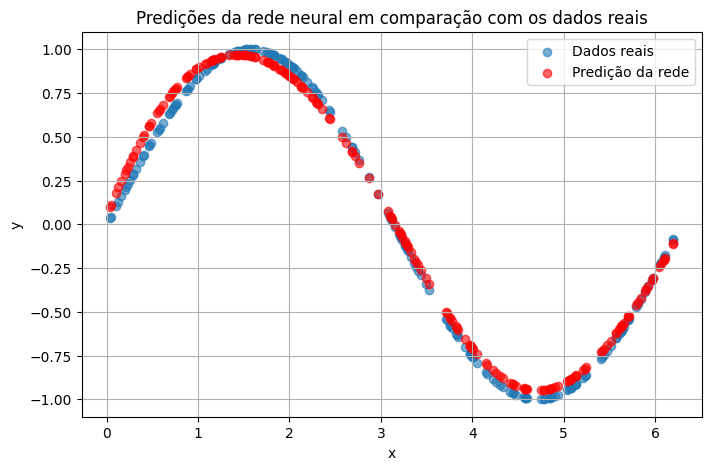
\includegraphics[width=\textwidth]{./0803_imgs/0365_tarefa05/png-241110-192904307-9336339325602212821.png}
		%\legend{Fonte: Gerado peloComando da atividade}
	\end{minipage}
	\hfill
	\begin{minipage}{0.45\textwidth}
		\centering
		\caption{$\sigma=0.1$}\label{fig:tarefa05:01:predicoes}
		
		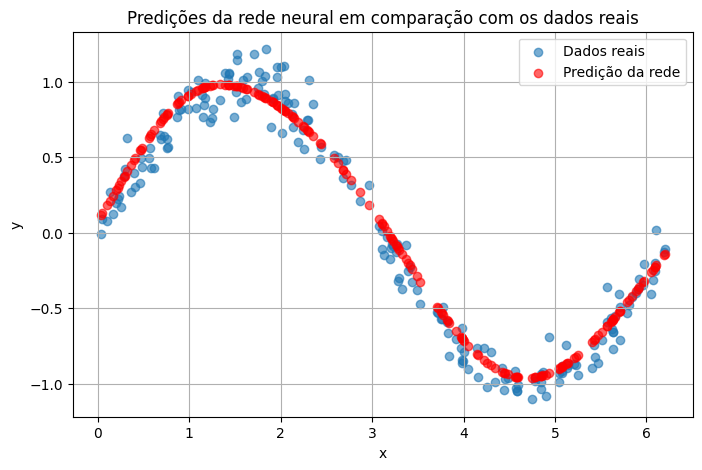
\includegraphics[width=\textwidth]{./0803_imgs/0365_tarefa05/png-241110-192925288-2928491021629715945.png}
		%\legend{Fonte: \citeonline[p. 24]{araujo2012}}
	\end{minipage}
	\vspace{2Ex}
	\begin{minipage}{0.45\textwidth}
		\centering
		\caption{$\sigma=0.3$}\label{fig:tarefa05:03:predicoes}
		
		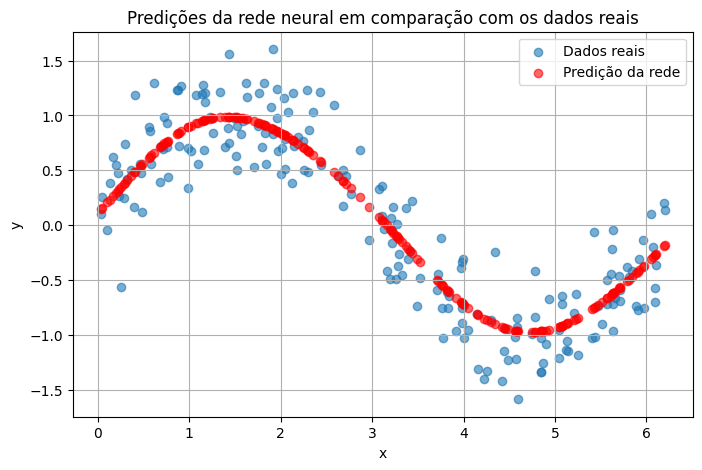
\includegraphics[width=\textwidth]{./0803_imgs/0365_tarefa05/png-241110-192954147-5354434943605266969.png}
		%		%\legend{Fonte: \citeonline[p. 24]{araujo2012}}
	\end{minipage}
	\hfill
	\begin{minipage}{0.45\textwidth}
		\centering
		\caption{$\sigma=0.5$}\label{fig:tarefa05:05:predicoes}
		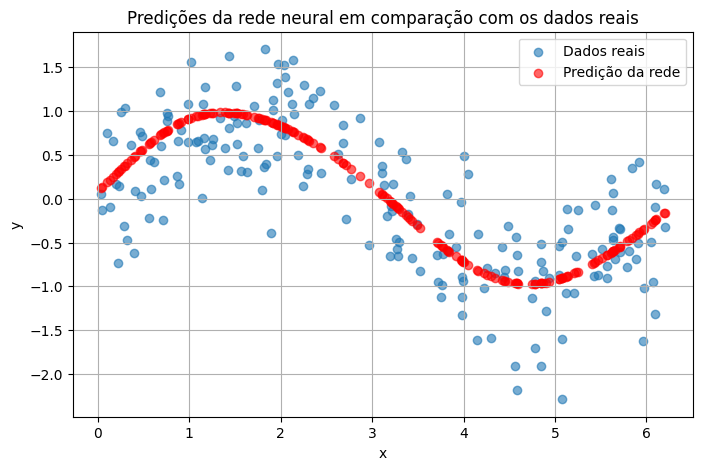
\includegraphics[width=\textwidth]{./0803_imgs/0365_tarefa05/png-241110-193141249-12530547749698557937.png}
		%\legend{Fonte: \citeonline[p. 24]{araujo2012}}
	\end{minipage}
\end{figure}



Em resumo, esta análise destaca a influência do ruído nos dados no processo de 
treinamento de modelos de aprendizado de máquina. Níveis mais altos de ruído 
podem levar a uma convergência mais lenta e instável, mas o modelo pode 
eventualmente adaptar-se e aprender a lidar com o ruído, como observado no caso 
de $\sigma=0,5$.
\subsection{Tarefa 06 -- Aplicação de Regularização L2}

\begin{comandoquestao}
Objetivo: Avaliar como a aplicação da regularização L2 ($\lambda_{L2}$) 
influencia o 
treinamento da rede neural, ajudando a prevenir o ``overfitting''. Exploraremos 
diferentes valores de lambda para entender seu impacto no desempenho da rede.
\end{comandoquestao}

Foram realizados experimentos de treinamento com quatro diferentes valores de 
$\lambda_{L2}$ (fator de regularização L2): 0,0, 0,001, 0,01 e 0,1. As curvas 
de treinamento são mostradas na \cref{fig:tarefas06:curvas}. As previsões da 
rede pode ser visualizadas nas 
\cref{fig:tarefa06:00:predicoes,fig:tarefa06:0001:predicoes,fig:tarefa06:001:predicoes,fig:tarefa06:01:predicoes}.


\begin{figure}[tbh]
	\centering
	\caption{Curvas de aprendizado para diferentes níveis de $\lambda_{L2}$}
	\label{fig:tarefas06:curvas}
	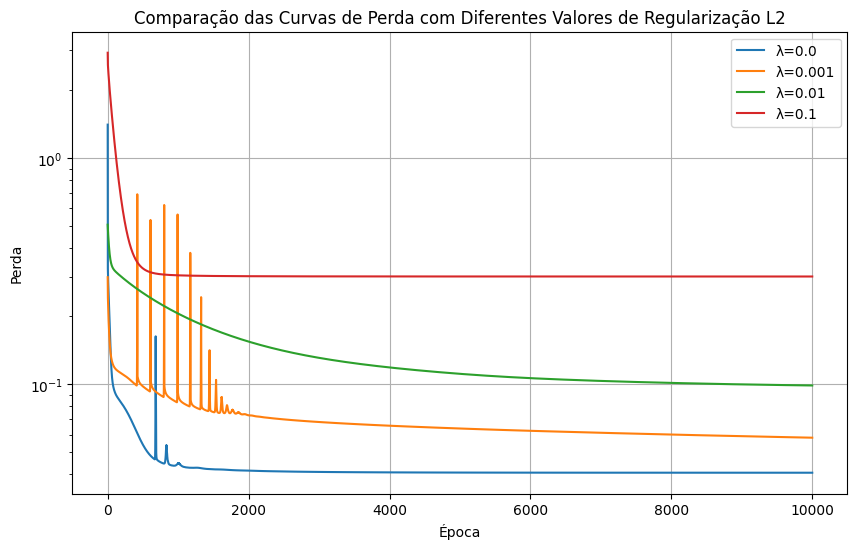
\includegraphics[width=0.7\linewidth]{./0803_imgs/0703_tarefa06/png-241113-093042368-16803966117590063962.png}
\end{figure}


\begin{figure}[htb]
	\centering
	\begin{minipage}{0.45\textwidth}
		\centering
		\caption{$\lambda_{L2}=0,0$}\label{fig:tarefa06:00:predicoes}
		
		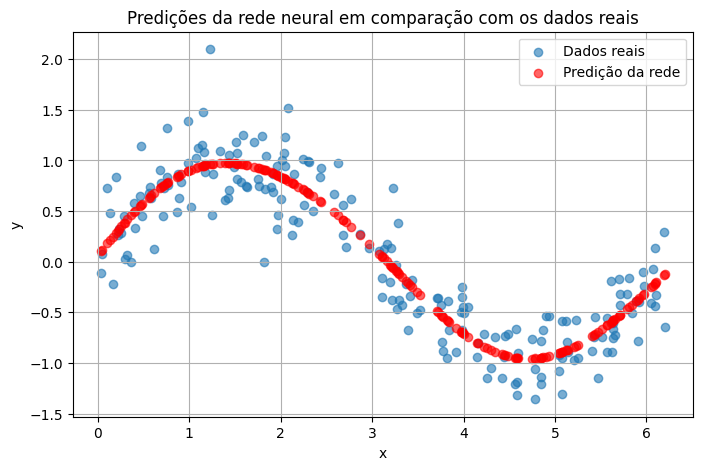
\includegraphics[width=\textwidth]{./0803_imgs/0703_tarefa06/png-241111-193408972-100508130524023774.png}
		%\legend{Fonte: Gerado peloComando da atividade}
	\end{minipage}
	\hfill
	\begin{minipage}{0.45\textwidth}
		\centering
		\caption{$\lambda_{L2}=0,001$}\label{fig:tarefa06:0001:predicoes}
		
		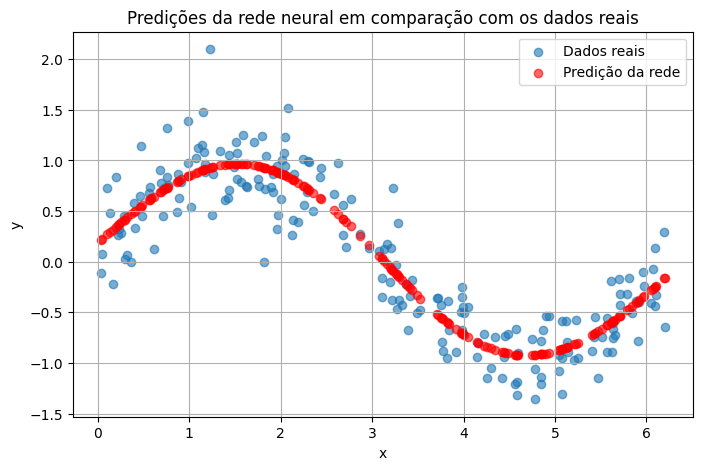
\includegraphics[width=\textwidth]{./0803_imgs/0703_tarefa06/png-241111-193433094-6903075368889255079.png}
		%\legend{Fonte: \citeonline[p. 24]{araujo2012}}
	\end{minipage}
	\vspace{2Ex}
	\begin{minipage}{0.45\textwidth}
		\centering
		\caption{$\lambda_{L2}=0,01$}\label{fig:tarefa06:001:predicoes}
		
		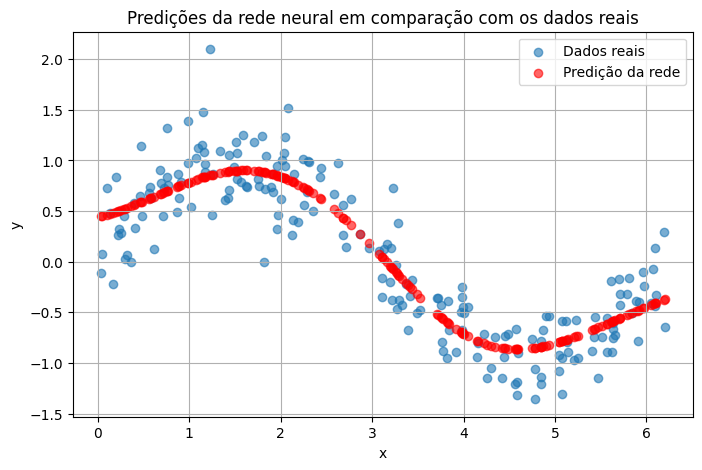
\includegraphics[width=\textwidth]{./0803_imgs/0703_tarefa06/png-241111-193629109-11720175723589392501.png}
		%		%\legend{Fonte: \citeonline[p. 24]{araujo2012}}
	\end{minipage}
	\hfill
	\begin{minipage}{0.45\textwidth}
		\centering
		\caption{$\lambda_{L2}=0,1$}\label{fig:tarefa06:01:predicoes}
		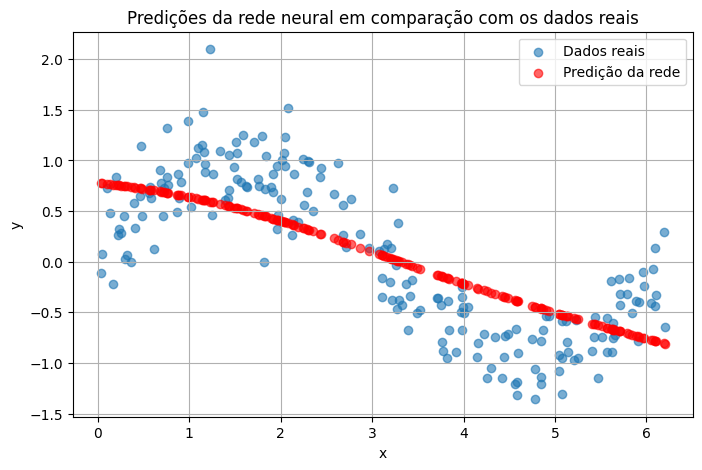
\includegraphics[width=\textwidth]{./0803_imgs/0703_tarefa06/png-241111-193757953-13380955252315067618.png}
		%\legend{Fonte: \citeonline[p. 24]{araujo2012}}
	\end{minipage}
\end{figure}

 Quando $\lambda_{L2}=0,0$, o que significa nenhuma regularização, o modelo 
 atinge uma perda de 0.04069 após 9900 épocas. Com $\lambda_{L2}=0,001$, um 
 pequeno valor de regularização é aplicado, e a perda 
aumenta para 0.05821. Isso indica que a regularização está tendo um efeito 
moderado no 
desempenho do modelo.

Quando $\lambda_{L2}=0.01$, a perda aumenta significativamente para 0.09901. 
Neste caso, o 
modelo está mostrando sinais de ``underfitting'', significando que a 
regularização é muito forte e começa a prejudicar a capacidade da rede de 
aprender padrões complexos. O comportamento é semelhante ao de um modelo 
treinado com poucas épocas, sugerindo que a regularização excessiva pode ter um 
efeito semelhante à falta de treinamento.

Para $\lambda_{L2}=0,1$, a perda aumenta drasticamente para 0.30001. Este valor 
alto de $\lambda_{L2}$ 
resulta em uma forte penalidade na complexidade do modelo, levando a um 
comportamento de previsão quase linear (\cref{fig:tarefa06:01:predicoes}). O 
modelo está sendo fortemente restrito 
e não consegue capturar a complexidade dos dados, resultando em um desempenho 
inferior.

Em resumo, esta análise destaca a importância de escolher o fator de 
regularização adequado. Uma regularização muito fraca pode levar a 
problemas de ``overfitting'', enquanto uma regularização muito forte 
($\lambda_{L2}=0.1$) 
pode 
resultar em ``underfitting'' e comportamento simplista. O valor de 
$\lambda_{L2}=0,001$ 
parece ser um bom equilíbrio, permitindo alguma regularização sem comprometer 
significativamente o desempenho do modelo. A escolha do fator de regularização 
ideal depende dos dados específicos e do nível de complexidade desejado do 
modelo.
\section{Conclusão}

Nesta presente análise, investigamos o impacto de vários parâmetros e 
hiperparâmetros no treinamento e desempenho de redes neurais. Exploramos 
diferentes funções de ativação, números de épocas, taxas de aprendizagem, 
arquiteturas de rede, níveis de ruído nos dados e taxa de regularização. 
Cada 
tarefa forneceu ``insight''s sobre como esses fatores influenciam o 
comportamento e a capacidade preditiva das redes neurais.

\begin{comment}
Na tarefa 1, descobrimos que a função de ativação Gelu nas camadas 
intermediárias resultou em uma melhor capacidade de aprendizado em 
comparação 
com a função sigmóide. A função Relu, embora interessante, apresentou um 
comportamento mais ruidoso, sugerindo a necessidade de uma inicialização 
de 
parâmetros e taxa de aprendizagem cuidadosas.

Na tarefa 2, observamos que um número excessivo de épocas de treinamento 
pode 
não trazer benefícios significativos após um certo ponto. As redes neurais 
convergiram para erros semelhantes após 5000 épocas, e a rede treinada com 
apenas 1000 épocas exibiu underfitting. Esta análise destaca a importância 
de 
monitorar o desempenho em diferentes pontos do treinamento.

A tarefa 3 enfatizou a escolha crucial da taxa de aprendizagem. Uma taxa 
muito 
baixa resultou em convergência lenta, enquanto uma taxa muito alta levou a 
um 
comportamento instável. A taxa de 0,05 pareceu ser um bom equilíbrio, 
proporcionando uma convergência suave e um bom desempenho final.

Na tarefa 4, descobrimos que a complexidade da arquitetura da rede deve 
ser 
considerada em relação à quantidade de dados. Uma rede neural mais simples 
pode 
convergir bem e fornecer resultados comparáveis a redes mais profundas, 
dependendo do problema.

A tarefa 5 revelou que níveis mais altos de ruído nos dados resultaram em 
uma 
convergência mais lenta e instável, mas o modelo adaptou-se e aprendeu a 
lidar 
com o ruído. Esta análise destaca a importância de considerar a qualidade 
dos 
dados e a necessidade de lidar com o ruído durante o treinamento.

Por fim, na tarefa 6, vimos que a regularização L2 pode ajudar a prevenir 
o 
overfitting, mas uma regularização muito forte pode levar a underfitting. 
O 
valor de λ=0.001 pareceu ser um bom equilíbrio, permitindo alguma 
regularização 
sem comprometer o desempenho.
\end{comment}

Esta série de tarefas demonstra a importância da seleção cuidadosa 
de parâmetros e hiperparâmetros no treinamento de redes neurais. A escolha 
adequada de funções de ativação, número de épocas, taxa de aprendizagem, 
arquitetura e regularização é crucial para alcançar um bom desempenho e 
evitar 
problemas como \textit{overfitting} e \textit{underfitting}. A análise 
sistemática desses 
fatores é essencial para otimizar os modelos de aprendizado de máquina e 
garantir sua capacidade de generalização para novos dados.
%
\section{Consulte o manual da classe \textsf{abntex2}}

Consulte o manual da classe \textsf{abntex2} \cite{abntex2classe} para uma
referência completa das macros e ambientes disponíveis.

% ---
% Finaliza a parte no bookmark do PDF, para que se inicie o bookmark na raiz
% ---
\bookmarksetup{startatroot}%
% ---

% ---
% Conclusão
% ---
\section{Considerações finais}

\lipsum[1]

\begin{citacao}
\lipsum[2]
\end{citacao}

\lipsum[3]

% ----------------------------------------------------------
% ELEMENTOS PÓS-TEXTUAIS
% ----------------------------------------------------------
\postextual

% ----------------------------------------------------------
% Referências bibliográficas
% ----------------------------------------------------------
\bibliography{abntex2-modelo-references}

% ----------------------------------------------------------
% Glossário
% ----------------------------------------------------------
%
% Há diversas soluções prontas para glossário em LaTeX.
% Consulte o manual do abnTeX2 para obter sugestões.
%
%\glossary

% ----------------------------------------------------------
% Apêndices
% ----------------------------------------------------------

% ---
% Inicia os apêndices
% ---
\begin{apendicesenv}

% ----------------------------------------------------------
\chapter{Nullam elementum urna vel imperdiet sodales elit ipsum pharetra ligula
ac pretium ante justo a nulla curabitur tristique arcu eu metus}
% ----------------------------------------------------------
\lipsum[55-56]

\end{apendicesenv}
% ---

% ----------------------------------------------------------
% Anexos
% ----------------------------------------------------------
\cftinserthook{toc}{AAA}
% ---
% Inicia os anexos
% ---
%\anexos
\begin{anexosenv}

% ---
\chapter{Cras non urna sed feugiat cum sociis natoque penatibus et magnis dis
parturient montes nascetur ridiculus mus}
% ---

\lipsum[31]

\end{anexosenv}

% ----------------------------------------------------------
% Agradecimentos
% ----------------------------------------------------------
\section*{Agradecimentos}
Texto sucinto aprovado pelo periódico em que será publicado. Último
elemento pós-textual.



\end{document}
